\documentclass[11pt]{amsart}
\usepackage{geometry}                % See geometry.pdf to learn the layout options. There are lots.
\geometry{letterpaper}                   % ... or a4paper or a5paper or ... 
%\geometry{landscape}                % Activate for for rotated page geometry
%\usepackage[parfill]{parskip}    % Activate to begin paragraphs with an empty line rather than an indent
\usepackage{graphicx}
\usepackage{amssymb}
\usepackage[square,numbers]{natbib}
\usepackage{amsmath, epsfig}
\usepackage{amsfonts}
\usepackage{amssymb}
\usepackage{subfigure}
\usepackage{graphicx}
\usepackage{amsfonts}
\usepackage{algorithm}
\usepackage{algorithmic}
\usepackage{easybmat}
\usepackage{footmisc}
\usepackage{lscape}
\usepackage{subfigure}
\usepackage{epstopdf}
\DeclareGraphicsRule{.tif}{png}{.png}{`convert #1 `dirname #1`/`basename #1 .tif`.png}

\title{Supervised Latent Dirichlet Allocation}
\author{Frank Wood and Adler Perotte (?)}
%\date{}                                           % Activate to display a given date or no date

\begin{document}
\maketitle

\section{Outline}
\subsection{MCMC}
\subsection{Auxiliary Variables}
\subsection{Probit Regression}

\begin{figure}[htbp]
\begin{center}
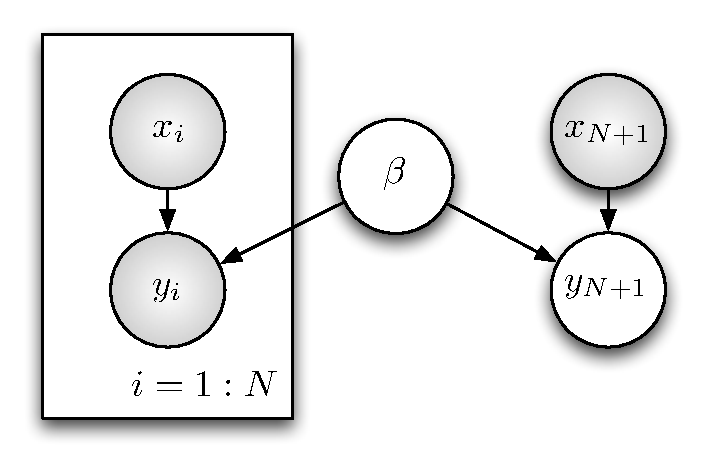
\includegraphics{probit_no_aux_vars}
\caption{Probit model, no auxiliary variables}
\label{fig:probit_no_aux_vars}
\end{center}
\end{figure}


\begin{figure}[htbp]
\begin{center}
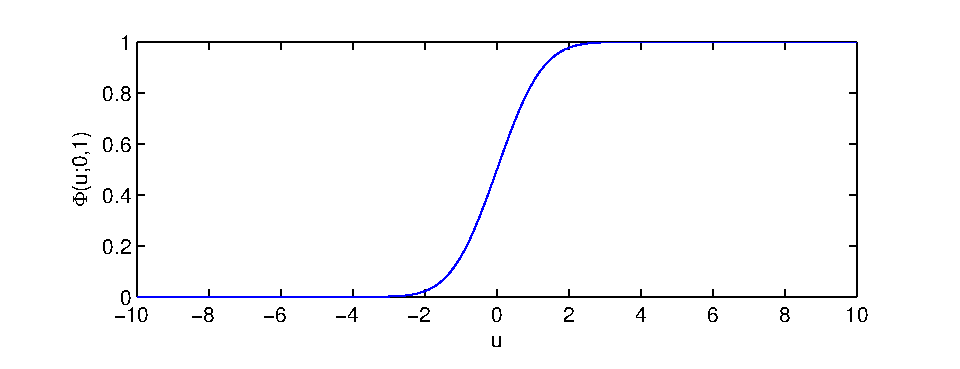
\includegraphics{cdf.eps}
\caption{CDF of $N(0,1)$}
\label{fig:cdf}
\end{center}
\end{figure}

\begin{figure}[htbp]
\begin{center}
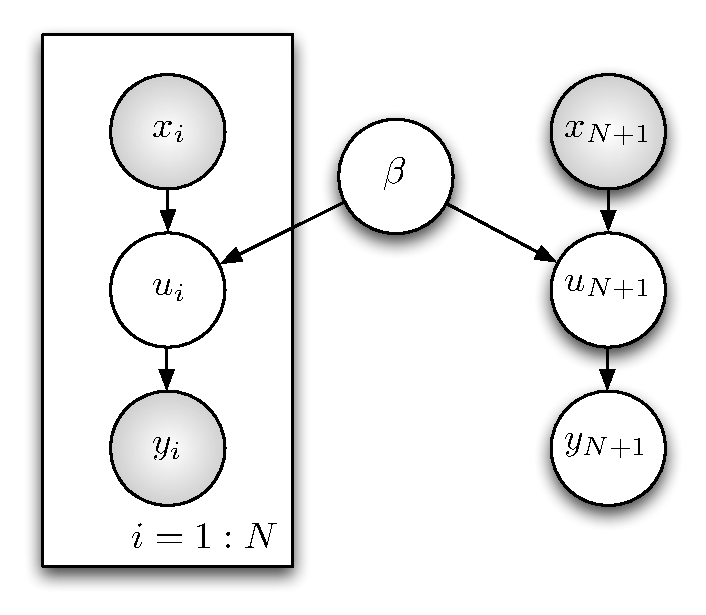
\includegraphics{probit}
\caption{Probit model}
\label{fig:probit}
\end{center}
\end{figure}




For reasons that are somewhat obscure to me, statisticians tend to use probit regression for binary classification whereas machine learners tend to use logistic regression.  In a recent paper, my collaborators and I found it useful for computational purposes to use probit regression.  One can find many good primers on probit regression around the web, but, as we all know, there is almost always space for another.  

Figure \ref{fig:cdf} is the cumulative distribution function (cdf) of a $N(0,1)$ distribution.  The ``probit'' function is the inverse of the normal cdf.    The normal cdf function, denoted $\Phi(x;\mu,\sigma^2)$ with $\mu$ the mean, $\sigma^2$ the variance and $x$ the argument, is actually much more relevant in this context.

The range of the normal cdf is $(0,1)$ which means that it can be interpreted as a probability.  For instance, one can construct a generalized linear model (a ``probit regression model'') of the form 
\begin{equation}
P(y_i = 1) = \Phi(x_i^T\beta; 0, \sigma^2). \label{eqn:probit}
\end{equation}  Depending on convention (i.e. binary $y_i$ represented as $\{1,0\}$ or $\{1,-1\}$) then the probability of $y_i$ being labeled the opposite way is $P(y_i = -1)$ or $P(y_i = 0) = 1 - P(y_i=1).$  Here $x_i$ is a vector of covariates, $\beta$ is a vector of weights, and $y_i$ is a single, binary valued response.  As always, the close relationship between regression and classification are in full display here : probit regression is a ``generalized linear {\em regression} model'' and a ``binary classifier.''

Figure \ref{fig:probit_no_aux_vars} shows the graphical model for probit regression (minus any priors on the regression weights $\beta$).    In this model we would like to use labeled training data, $\{x_i, y_i\}_{i=1}^N$ to ``learn'' the value of $\beta$ and then to use this value to predict the value of $y_{N+1} | x_{N+1}, \beta.$  We will be being Bayesian about our inference so here, what we really mean is, we will average over the posterior distribution of $\beta$ when making predictions.  This means that we want to draw samples from the posterior distribution of $\beta | \{x_i, y_i\}_{i=1}^N$.  This brings us to Figure \ref{fig:probit} which introduces a set of auxiliary variables $\{u_i\}_{i=1}^N$.  In this note we will demonstrate that the model in  Figure \ref{fig:probit} is the same as the model in Figure \ref{fig:probit_no_aux_vars}  when the $u_i$'s are marginalized out and will suggest that inference in the former is computationally easier.  

First -- what is an auxiliary variable?  It is a variable introduced into a model in order to make inference easier but whose existence does not change the distribution of interest.  Auxiliary variables for slice sampling are one particularly clever use of auxiliary variables.  The auxiliary variable trick in probit regression is another.

For the purposes of exposition, let's forget about the $i$ index for a second and focus on a single instance $y$, $x$, and $u$.  The argument we make will hold for all by simply reintroducing subscripts.  

To start, let's write down the joint distribution of these quantities (according to the graphical model that includes auxiliary variables).

\begin{equation}
P(y,x,u) = P(y|u)P(u|x,\beta) \label{eqn:joint}
\end{equation}

Clearly, straight away, one can see precisely why this auxiliary variable scheme works.  By the law of total probability we have
\begin{equation}
P(y,x) = \int P(y,x,u)du= \int P(y|u)P(u|x,\beta)du.  \label{eqn:joint_marginalized}
\end{equation}
If by MCMC we generate $S$ samples $\{u^{(s)},y^{(s)},x^{(s)}\}_{s=1}^S \sim P(y,x,u)$ we know that marginalizing $u$ out (i.e.~disregarding its value) we get samples $\{y^{(s)},x^{(s)}\}_{s=1}^S \sim P(y,x).$  %Equation  \ref{eqn:joint_marginalized} 
%\begin{eqnarray}
%y_i &\sim& \Phi(x_i^T\beta; 0, 1)
%\end{eqnarray}

We haven't specified the most important part of the auxiliary variable sampling scheme yet, namely, what $P(y|u)$ and what $P(u|x,\beta)$ are.   Let's try $y = \mbox{sign}(u)$ and $u \sim N(x^T\beta,\sigma^2).$  These choices are nice in a particular way.  First let's verify that the marginalization of $u$ out of this model results in the model specification in Equation \ref{eqn:probit}.

\begin{eqnarray*}
P(y=1|x,\beta) &=&  \int P(y=1|u)P(u|x,\beta)du\\
&=& \int \mathbb{I}(u>0)N(u;x^T\beta,\sigma^2) du \\
&=& \int_0^\infty N(u;x^T\beta,\sigma^2) du \\
&=& 1 - \Phi(0; x^T\beta,\sigma^2) \\ 
&=& \Phi(x^T\beta; 0, \sigma^2)
\end{eqnarray*}
where the last line comes from the fact that for symmetric distributions like the normal distribution, 
$\Phi(x^T\beta; 0, \sigma^2) = 1 - \Phi(-x^T\beta; 0, \sigma^2)$ and the mean of a normal cdf can be translated arbitrarily, i.e. $\Phi(-x^T\beta; 0, \sigma^2) = \Phi(0;x^T\beta, \sigma^2)$ (which comes from adding the offset $x^T\beta$ to the cdf argument and mean).  

OK.  So, now, we have established the fact that for a particular sort of auxiliary variable choice, we get the same probit model as we wanted.  Why is this choice nice?

Well, it comes down to sampling $\beta$ and $u$ and $y$.  Generally, sampling $\beta$ in the model without auxiliary variables will require hybrid Monte Carlo (HMC) or Metropolis Hastings of some sort.  Gibbs sampling often comes with substantial benefits.  By making this choice of auxiliary variable the conditional distribution of $u_i$ given everything else is proportional to a truncated Normal distribution, a distribution that is, by nature of its commonness, relatively straightforward to sample from.  The big benefit, though, acrues from the posterior form for sampling $\beta$.  With the $u$'s ``observed'' (as they would be in a Gibbs sampler), the posterior distribution of $\beta$ (for typical choices of prior) is precisely the same as that for linear regression, perhaps the most well studied model in statistics.  Sampling $\beta$ from its posterior distribution typically is quite simple; certainly more so that sampling $\beta$ without the $u$ auxiliary variables.


\subsection{LDA}
\subsection{sLDA}
\subsection{hsLDA}
\subsection{Experiments}


\section{Background}
There are many 

%\subsection{}
\section{Introduction}
\label{sec:introduction}
% !TEX root = main.tex
\section{Introduction}
\label{section_introduction}

Predictive models are all about doing as much as you can with as little data and computation as possible.  If sufficient for application purposes, resorting to simple models is often effective.  

Richly expressive models require   

Bayesian approaches to prediction dictate tying and sharing parameters, often through hierarchies and so forth. 

Cite 

Related work on multiscale language modeling
\citep{Goldwater2009,Mochihashi2009}

Related work on transformed Dirchlet processes and HDP's with random effects.
\citep{Sudderth2005,Kim2007,Hoffman2009,}

\section{Model}
\label{sec:model}
\section{Bayesian PDFA Inference}

The outline of this section is as follows.  We define a prior distribution over PDFAs with a fixed number of states and show that many of the parameters can be integrated out.  We derive a Metropolis-Hastings sampler for posterior inference in the finite model, and show that many of the elements of the transition matrix can be ignored without affecting the correctness of sampling.  We then let the number of states go to infinity and show that the limit is well defined.  This is the probabilistic deterministic infinite automaton (PDIA).  Inference in the PDIA carries over from the finite case in a natural way.

\subsection{A Prior over PDFAs}

We assume that the states $Q$, alphabet $\Sigma$ and initial state $q_0$ are known, and define a prior over the transition function $\delta$ and emission probabilities $\pi$.  In the finite case $\delta$ and $\pi$ can be thought of as matrices, with columns indexing elements of $\Sigma$ and rows indexing elements of $Q$.  For each column $j$ of the transition matrix $\delta$, we sample the rows i.i.d. from a discrete distribution $\bphi_j$ over $Q$, that is, $\delta \sim [\bphi_1\ldots\bphi_{|\Sigma|}]$.  The $\bphi_j$ themselves are sampled i.i.d. from a Dirichlet prior with parameters $\alpha\bmu$, where $\alpha$ is a concentration and $\bmu$ is itself drawn from a uniform Dirichlet distribution, with $\gamma$ total pseudocounts.  This hierarchical Dirichlet construction allows elements of $\delta$ to be coupled together in a way that remains well-behaved in the limit of infinite states.  We also place a uniform Dirichlet prior over the per-state emission probabilities $\bpi_i$ with $\beta$ total pseudocounts.  Formally:

\begin{eqnarray}
\bmu|\gamma,|Q| & \sim & \mathrm{Dir}\left(\gamma/|Q|,\ldots,\gamma/|Q|\right) \label{gen:mu} \\
\bphi_{j}|\alpha,\bmu  & \sim & \mathrm{Dir}(\alpha\bmu) \label{gen:phi} \\
\bpi_{i}|\beta,|\Sigma| & \sim & \mathrm{Dir}(\beta/|\Sigma|,\ldots,\beta/|\Sigma|) \label{gen:pi}\\
\delta_{ij} & \sim & \bphi_{j} \label{gen:delta}
\end{eqnarray}

where $i$ goes from 0 to $|Q|-1$ and $j$ goes from 1 to $|\Sigma|$.  From this we generate a sequence of $T$ symbols:

\begin{eqnarray}
\q_0 & = & q_0 \label{gen:q0} \\
x_0 & \sim & \bpi_0 \label{gen:x0} \\
\q_t & = & \delta(\q_{t-1},x_{t-1}) \label{gen:q} \\
x_t & \sim & \bpi_t \label{gen:x}
\end{eqnarray}

We choose this particular inductive bias, with transitions tied together within a column of $\delta$, because the most recent symbol ought to be informative about what the next state is.  If we instead had a single Dirichlet prior over all elements of $\delta$, transitions to a few states would be highly likely no matter the context and those states would dominate the behavior of the automata.  If we tied together rows of $\delta$ instead of columns, being in a particular state would tell us more about the sequence of states we came from than the symbols that got us there.  As we would like states to be good statistics of the past for predicting the future, a bias that depends on the most recent symbol is preferable.

Given data, the likelihood is

\[ p(x_{0:T}|\delta,\pi) = \pi(\q_0,x_0)\prod_{t=1}^T \pi(\q_t,x_t) \label{x:def} \]

We can marginalize out $\pi$ and express the likelihood in a form that depends only on the counts of symbols emitted from each state.  Define the count matrix $c$ for the sequence $x_{0:T}$ and transition matrix $\delta$ as $c_{ij} = \displaystyle\sum_{t=0}^T I_{ij}(\q_t,x_t)$, where $I_{ij}(\q_t,x_t)$ is an indicator function that is 1 if $\q_t = q_i$ and $x_t = \sigma_j$, 0 otherwise. This matrix gives the number of times each symbol is emitted from each state.  Thanks to multinomial-Dirichlet conjugacy we can integrate out $\pi$ and express the probability of a sequence given the transition function $\delta$ solely in terms of $c$ and $\beta$:

\begin{eqnarray}
 p(x_{0:T}|\delta,\beta) & = & \int p(x_{0:T}|\pi,\delta) p(\pi|\beta) d\pi \label{x:factor} \\
 & = &  \prod_{i=0}^{|Q|-1} \frac{\Gamma(\beta)}{\Gamma(\frac{\beta}{|\Sigma|})^{|\Sigma|}} \int\pi_{i1}^{\frac{\beta}{|\Sigma|}+c_{i1}-1} \pi_{i2}^{\frac{\beta}{|\Sigma|}+c_{i2}-1} \ldots \pi_{i|\Sigma|}^{\frac{\beta}{|\Sigma|}+c_{i|\Sigma|}-1} d\bpi_i \label{x:int}\\
 & = & \prod_{i=0}^{|Q|-1} \frac{\Gamma(\beta)}{\Gamma(\frac{\beta}{|\Sigma|})^{|\Sigma|}} \frac{\prod_{j=1}^{|\Sigma|}\Gamma(\frac{\beta}{|\Sigma|} + c_{ij})}{\Gamma(\beta + \sum_{j=1}^{|\Sigma|} c_{ij})} \label{x:end}
 \end{eqnarray}
 
 The dependence of $c$ on $\delta$ is only through $\q_{0:T}$, and changing a single element of $\delta$ can have a complex effect on $c$.  By changing a single transition $\delta_{ij}$, all states downstream of the first time $q_i$ emits $\sigma_j$ are affected, and some elements of $c$ that were zero may become nonzero, and vice versa.
 
 The likelihood of a particular transition matrix $\delta$ given $\bmu$ has a similar form.  Let $v_{ij}$ be the number of times that $\delta_{i'j} = q_i$ for all $i'$ in the column $j$, that is, $v_{ij} = \displaystyle\sum_{i' = 0}^{|Q|-1} I_{i}(\delta_{i'j})$, $I_i(q_{i'})$ being the indicator function that is only 1 when $q_i' = q_i$.  Given $\bmu$, we can integrate out $\phi$ and express the likelihood of $\delta$ in terms of $\bmu$:
 
 \begin{eqnarray}
 p(\delta|\bmu,\alpha) & = & \int p(\delta|\phi)p(\phi|\bmu,\alpha) d\phi \label{delta:factor}\\
  & = & \prod_{j=1}^{|\Sigma|} \frac{\Gamma(\alpha)}{\prod_{i=0}^{|Q|-1}\Gamma(\alpha\mu_i)} \int \phi_{0j}^{\alpha\mu_0+v_{0j}-1} \phi_{1j}^{\alpha\mu_1+v_{1j}-1} \ldots \phi_{|Q|-1,j}^{\alpha\mu_{|Q|-1}+v_{|Q|-1,j}-1} d\bphi_j \label{delta:int}\\
  & = &  \prod_{j=1}^{|\Sigma|} \frac{\Gamma(\alpha)}{\prod_{i=0}^{|Q|-1}\Gamma(\alpha\mu_i)} \frac{\prod_{i=0}^{|Q|-1} \Gamma(\alpha\mu_i + v_{ij})}{\Gamma(\alpha + |Q|)} \label{delta:end}
  \end{eqnarray}

%Finally, the posterior probability of $\bmu$ given $\delta$ is

%\begin{eqnarray}
%p(\bmu|\delta,\alpha, \gamma) & = & \frac{p(\delta|\bmu,\alpha)p(\bmu|\gamma)}{\int p(\delta|\bmu,\alpha)p(\bmu|\gamma) d\bmu}
%\end{eqnarray}

These are the ingredients we need for posterior inference.
 
 \subsection{Posterior Inference in the Finite Model}
 
We perform posterior inference in the finite model by Gibbs sampling elements of $\delta$ and the vector $\bmu$.  From the formulas above, it is straightforward to write down the conditional probability for one element of the transition matrix $\delta$.  If $\delta_{ij}$ is the element we are sampling, and $\delta_{-ij}$ is the rest of the matrix, with $\delta_{ij}$ removed, then

\begin{equation}
p(\delta_{ij}|\delta_{-ij},x_{0:T},\bmu,\alpha) \propto p(x_{0:T}|\delta_{ij},\delta_{-ij})p(\delta_{ij}|\delta_{-ij},\bmu,\alpha) \label{delta:cond}
\end{equation}

Both terms on the right hand side of this equation have closed-form expressions, the first given in \eqref{x:end}.  The second can be found from \eqref{delta:end} to be

\begin{equation}
P(\delta_{ij} = q_{i'}|\delta_{-ij},\alpha,\bmu) = \frac{\alpha\mu_{i'} + v_{i'j}}{\alpha + |Q| - 1} \label{delta:pred}
\end{equation}

Where $v_{i'j}$ is the number of elements in column $j$ equal to $q_{i'}$ {\em excluding} $\delta_{ij}$.  As $|Q|$ is finite, we can construct and normalize the conditional probability vector for $\delta_{ij}$ and sample.

We can simplify inference by ignoring transitions $\delta_{ij}$ for which the corresponding count $c_{ij}$ are 0.  Note that the likelihood of the data on the right hand side of \eqref{delta:cond} does not depend on $\delta_{ij}$ if $c_{ij} = 0$, so sampling conditioned on the data is the same as sampling without conditioning on the data.  Thus, if changing some other transition means $c_ij$ becomes 0, we can remove $\delta_{ij}$ until another transition is changed so the count again is nonzero, and we sample a new value for $\delta_{ij}$ from \eqref{delta:pred}, just as we would have during Gibbs sampling had we not removed it.  Note that the joint distribution over a column of $\delta$ is exchangeable, and so removing an observation is the same as marginalizing it out, meaning that sampling the other elements of $\delta$ is still correct, but now conditioned on the model where superfluous transitions are marginalized out.  When we remove multiple elements from a column of $\delta$, we have to replace the $|Q| - 1$ in the denominator of \eqref{delta:pred} with $K^+_j = \sum_{i=0}^{|Q|-1}v_{ij} \leq |Q|$, the number of entries in the $j$th column of $\delta$ that are {\em not} marginalized out.

The posterior for $\bmu$ up to a normalization constant is

\begin{eqnarray}
p(\bmu|\delta,\alpha,\gamma) & \propto & p(\bmu|\gamma) p(\delta|\bmu,\alpha)\nonumber \\
& = & \frac{\Gamma(\gamma)}{\Gamma(\frac{\gamma}{|Q|})^{|Q|}}(\mu_1\ldots\mu_{|Q|})^{\frac{\gamma}{|Q|}-1}\prod_{j=1}^{|\Sigma|} \frac{\Gamma(\alpha)}{\prod_{i=0}^{|Q|-1}\Gamma(\alpha\mu_i)} \frac{\prod_{i=0}^{|Q|-1} \Gamma(\alpha\mu_i + v_{ij})}{\Gamma(\alpha + K^+_j)}
\end{eqnarray}

We can sample this by Metropolis-Hastings, for example using Dir($\eta\hat\bmu$) as the proposal, where $\hat\bmu$ is our current estimate and $\eta$ is a large concentration parameter, or take the MAP estimate as in \cite{Mackay1995}.  Fortunately in the infinite limit a more natural way to sample presents itself.
 
 \subsection{The Probabilistic Deterministic Infinite Automaton}
 
 We now consider what happens when $|Q|\rightarrow\infty$.  Given a finite amount of data, there can only be nonzero counts for a finite number of state/symbol pairs, so we can marginalize out all but at most $T$ elements of $\delta$.  Denote these active entries by $\delta^T$.  The predictive probability for a new $\delta_{ij} = q_{i'}$ given $\delta^T$ is given by $\frac{\alpha\mu_{i'} + v_{i'j}}{\alpha + K^+_j}$.  Note that this only depends on $|Q|$ through $\mu_{i'}$, which is well behaved as $|Q|$ grows.  In the limiting case, most of the mass of $\bmu$ will concentrate on a handful of elements, and $\bmu$ becomes a draw from a {\em Dirichlet process} (DP), which is commonly used as a prior in Bayesian models with infinite parameters.  The hierarchical Dirichlet construction given in \eqref{gen:mu} and \eqref{gen:phi} becomes a {\em hierarchical Dirichlet process} (HDP), where the $\bphi_j$ are draws from a Dirichlet process whose parameters are given by $\alpha$ and $\bmu$, which is itself a draw from a Dirichlet process.  An attractive property of HDPs is that both the $\bphi_j$ and $\bmu$ can be integrated out, which makes sampling more straightforward than in the finite case.  This  representation of the model, with all draws from a DP integrated out, is known as the {\em Chinese Restaurant Franchise} (CRF).  This curious name needs some explanation, which we happily provide.
 
%We can sample incrementally from the joint distribution over $x_{0:T}$ and $\delta$ when $\phi_j$, $\mu$ and $\pi_i$ are integrated out in the $|Q|\rightarrow\infty$ limit.  From the start state $q_0$, we sample a symbol $s_{j_0}$ uniformly and assign $\delta_{0j_0}$ to a new state.  If $q^t = q_i$ then $x_t$ has the probability

% \[P(x_t=s_j|q_i,x_{0:t-1},q^{0:t-1}) = \frac{c_{ij}+\frac{\beta}{|\Sigma|}}{c_{i\cdot} + \beta}\]
 
% where $c_{ij}$ is the number of times so far $s_j$ was emitted from $q_i$ and $c_{i\cdot}$ is the total number of times $q_i$ has been visited so far.  
 
%If the state/symbol pair $(q_i,s_j)$ has not been visited before, we have to sample $\delta_{ij}$.  The two-stage generative procedure for elements of $\delta$ means that we have to keep track of counts at two levels.  Each $\delta_{ij}$ belongs to a cluster $v_{kj}$ that contains other $\delta_{i'j}$, while each $v_{kj}$ belongs to a top-level cluster $w_{l}$ that has elements across all $j$.  Each top level cluster has one $q \in Q$ assigned to it, and $\delta_{ij}$ is equal to that $q$ in the top cluster that the cluster with $\delta_{ij}$ belongs to (*might want to make this part clearer...add a figure*).  Let $\delta^t$ denote the elements of $\delta$ that have been visited at time $t$.  as follows:
 
%\[P(\delta_{ij} = k|\delta^t) \propto \begin{cases} & if $k \leq |\delta^t|$ \cr  & if $k > |\delta^t|$ \end{cases}\]
 
% This process for sampling from an HDP when $\mu$ and $\phi_j$ are integrated out is known as the {\em Chinese Restaurant Franchise Process}.

\section{Inference}
\label{sec:inference}
 \section{Posterior Inference over PDFAs}
 
 We perform posterior inference by sampling assignments for $\delta_{ij}$ individually.  Rather than ordinary Gibbs sampling, we use a mixed Gibbs/Metropolis-Hastings update.  To see why, consider the following case:  $\delta_{ij}$ is the only sampled element of $\delta$ that is assigned to the state $q_{i'}$.  When we removed $\delta_{ij}$ from the counts to sample it, the probability of assigning it back to $q_{i'}$ becomes zero, and even if it is assigned to some new state $q_{i''}$, the probability that $\delta_{i'j} = \delta_{i''j}$ for all $j$ visited by the data is low.  We do not want to forget a good sample, so instead we propose a new $\delta_{ij}$ and accept or reject according to the usual Metropolis-Hastings ratio.
 
Samples from the CRF are exchangeable, so we can remove $\delta_{ij}$ and propose a sample $\delta{ij}^*$ according to the CRF given $\delta_{-ij}^T$, the elements of $\delta$ visited by $x_{0:T}$ excluding $\delta_{ij}$.  This is the prior probability excluding the data, which cancels with the equivalent term in the posterior, meaning that the accept probability $\alpha(\delta_{ij},\delta_{ij}^*)$ is given by the ratio of the likelihood of the data

\[ \alpha(\delta_{ij},\delta_{ij}^*) =  \mathrm{min}\left(1,\frac{p(x_{0:T}|\delta_{ij}^*,\delta_{-ij}^T)}{p(x_{0:T}|\delta_{ij},\delta_{-ij}^T)}\right)\]

In general the numerator cannot be evaluated because changing $\delta_{ij}$ means changing the entire sequence of states visited by the data after $\delta_{ij}$ is first visited.  In practice we estimate the numerator by Monte Carlo approximation, sampling elements of $\delta$ according to the CRF as they are first visited by the data.  Changing one element of $\delta$ means many already-sampled state/symbol pairs may never be visited by the data, and have no effect on the likelihood.  The posterior probability of any value for these elements of $\delta$ is the same as the prior, and therefore we may remove them from $\delta^T$ after accepting a new $\delta_{ij}$.
section{Related Work}

\label{sec:related_work} 
In this work we extend supervised latent Dirichlet allocation (sLDA)
\cite{BleiMcAuliffe2008} to take advantage of hierarchical supervision. sLDA
is latent Dirichlet allocation (LDA) \cite{Blei2003} augmented with per
document ``supervision,'' often taking the form of a single numerical or
categorical label. It has been demonstrated that the signal provided by such
supervision can result in better, task-specific document models and can also
lead to good label prediction for out-of-sample data \cite{BleiMcAuliffe2008}.
It also has been demonstrated that sLDA has been shown to outperform both LASSO
(L1 regularized least squares regression) and LDA followed by least squares
regression~\cite{BleiMcAuliffe2008}. sLDA can be applied to data of the type
we consider in this paper; however, doing so requires ignoring the hierarchical
dependencies amongst the labels. In Section~\ref{sec:experiments} we constrast
HSLDA with sLDA applied in this way. 

%While there has been much work in multi-label classification of text and
%text modeling in general, we focus here on topic modeling approaches.
%Latent Dirichlet allocation (LDA) is a generative probabilistic model which
%represents documents as a mixed-membership bag of word. Each document is
%represented as a collection of words, generated from a set of topic assignments
%(one for each word), where each topic assignment is drawn from a distribution
%over topics~\citep{Blei2003}. sLDA is latent Dirichlet allocation (LDA)
%\cite{Blei2003} augmented with per-document labeling, often taking the form of
%a single numerical or categorical label. Examples of labels include ratings
%associated with online reviews, grades for essays, and the number of times a
%webpage is linked. This approach has been shown to outperform both LASSO
%(L1 regularized least squares regression) and LDA followed by least
%squares regression~\cite{BleiMcAuliffe2008}.

%Latent dirichlet allocation (LDA) is a generative
%probabilistic model of corpora that represents documents as a mixed
%membership bag-of-words. Also known as topic models, these models
%infer the latent structure, or topics, of documents in a corpus. Each
%document is represented as a collection of words, generated from a
%set of topic assignments (one for each word), where each topic assignment
%is drawn from a distribution over topics \citep{Blei2003}.

%Supervised latent Dirichlet allocation (sLDA) builds on LDA by incorporating
%supervision in the form of an observed exponential family response 
%variable per document. As a result, sLDA
%infers topics such that the model predicts the response variable while
%improing word likelihood.  This approach has been shown to outperform both LASSO
%(L1 regularized least squares regression) and LDA followed by least
%squares regression \citep{BleiMcAuliffe2008}.

Other models that incorporate LDA and supervision include
LabeledLDA~\citep{Ramage2009} and DiscLDA~\citep{DiscLDA}.  Various applications of these models to 
computer vision and document networks have been explored~\citep{wangbleifeifei08,RelationalLDA} .
None of these models, however, leverage dependency structure in the label space.

In other work, researchers have classified documents into a hierarchy (a closely related task) with naive Bayes classifiers
and support vector machines. Most of this work has been demonstrated on relatively
small datasets, small label spaces, and has focused on single label classification without
a model of documents such as LDA~\citep{mccallum99building,Dumais2000HCW,Kollerilprints291,Chakrabarti1998SFS}.

%One set of models that are particularly relevant to HSLDA are Chang
%and Blei's hierarchical models for document networks (Relational Topic
%Models). In that family of models, they encountered a similar scenario
%where the lack of a link did not truly indicate absence. In hierarchically
%labeled data, negative labels are uncommon and the lack of a label
%in the hierarchy is not equivalent to a negative label. Therefore,
%as in the work of Chang and Blei, we employ regularization to account
%for the lack of negative labels. This will be discussed further in

% Noemie: check out what I wrote here, because I am not really sure this is
% correct. 
%There have been several models that incorporate both latent models of text and
%some form of
%supervision~\citep{Ramage2009,DiscLDA,wangbleifeifei08,RelationalLDA}. One set 
%of models that are particularly relevant to HSLDA are Chang and Blei's
%hierarchical models for document networks (Relational Topic Models). In that
%family of models, they encountered a similar scenario where an unselected label 
%does not always indicate absence. In hierarchical labels, this phenomenon is
%even more pervasive -- there are no explicit negative labels, but it is also
%unclear how to treat the parents of selected labels. Like in the work of Chang
%and Blei, we employ regularization to account for the lack of negative
%labeling. In our experiments, we look at the impact of assigning positive and
%negative instances to the ancestors of selected labels.


\section{Experiments}

\label{sec:experiments}
% !TEX root = deplump.tex
\section{Experiments}
\label{sec:experiments}

As the performance of batch deplump was established relative to other lossless compressors for a variety of datatypes in \citep{Gasthaus2010}, we focus our experiments on establishing a) that the approximations to inference in the sequence memoizer combined in this paper in order to make deplump a streaming compressor do not significantly adversely affect compression performance, b) that the resulting compressor can indeed compress extremely long sequences as the asymptotic guarantees would suggest it should, and c) what settings of the approximation parameters produce the best compression performance.

Before testing the algorithm on streaming corpus we compared the algorithm to batch deplump.  We compressed the 100Mb Wikipedia corpus used for the Hutter Prize \citep{Hutter2006} using the streaming variant of deplump with $L = 10^{7}$ and $D = 16$ and found it gives a compression ratio of 4.78.  Using batch deplump gives a compression ratio of 4.82 \citep{Gasthaus2010}, while running batch deplump repeatedly on the 5Mb subsections of the corpus reduces the compression ratio to 4.25.  These results demonstrate that the approximations made for streaming deplump give it a significant advantage over compressing the file in chunks and have very little negative effect when compared to the full model.

All of the experiments included in this paper use a complete Wikipedia text content dump \citep{Wikipedia} as a test corpus (26.8Gb uncompressed, 7.8Gb gziped and ??Gb paq9a'ed, each with default parameters, and 3.9Gb deplumped).  To establish what approximation parameters produce the best compression results we first ran streaming deplump on the first 100Mb section of the corpus limiting the depth to two different values ($D=16$ and $D=1024$) with a fixed limit on the number of nodes in the tree ($L=10^6$).  We observed that in both cases only very few nodes had high total counts ($c > 8,192$) suggesting that it might be possible to set the count upper bound to a relatively low value ($k= 8,192$) without significant compression performance degradation.  %That compression performance should not be affected by a reasonable count bound follows intuitively from the fact that in byte sequences $|\Sigma| = 256$ and setting $k=10,000$ is similar in effect to using 10,000 observations to estimate a 256 element discrete distribution.  
To ensure that compression performance did in fact not suffer, we compressed ten 100Mb subsections of the corpus (sampled randomly with replacement) for multiple values of $k$ between 128 and 32,768 (fixing $L=10^6$ and $D=16$).  We observed that average compression performance varied insignificantly over $k$ for $2^7 \leq k \leq s^{15}$.

 In each of the following experiments, subsections of the corpus were sampled with replacement.  In the first experiment the sampled subsections were all of size 100Mb, while in the second the sampled subsections varied in length.  In the first experiment, the interplay between limiting the number of nodes in the tree and restricting the depth of the tree was explored (results for which are shown in Figure~\ref{fig:varying_depths}).  Here $k$ was set to 8,192, while $L$ and the depth of the tree $D$ were varied as indicated in the figure.  In the second experiment, the interplay between stream length and node limit was explored (Figure~\ref{fig:varying_stream_length}).  In this experiment $k$ remained fixed at the same value and the depth was set to $D=16$ while $L$ varied as shown in the figure.  

Figure~\ref{fig:varying_depths} indicates that compression performance becomes essentially indistinguishable for depth restrictions greater than $D=10$.  However, this figure also suggests that compression performance almost always improves as a function of the number of nodes in the tree for depths 6 and greater.  Figure~\ref{fig:varying_stream_length} illustrates that the algorithm not only scales to very long sequences, but average compression performance continues to improve as the sequence grows.  Using a large value of $L$ appears to be beneficial for very long sequences.

\begin{figure*}[t] 
	\begin{center}
		\scalebox{.6}{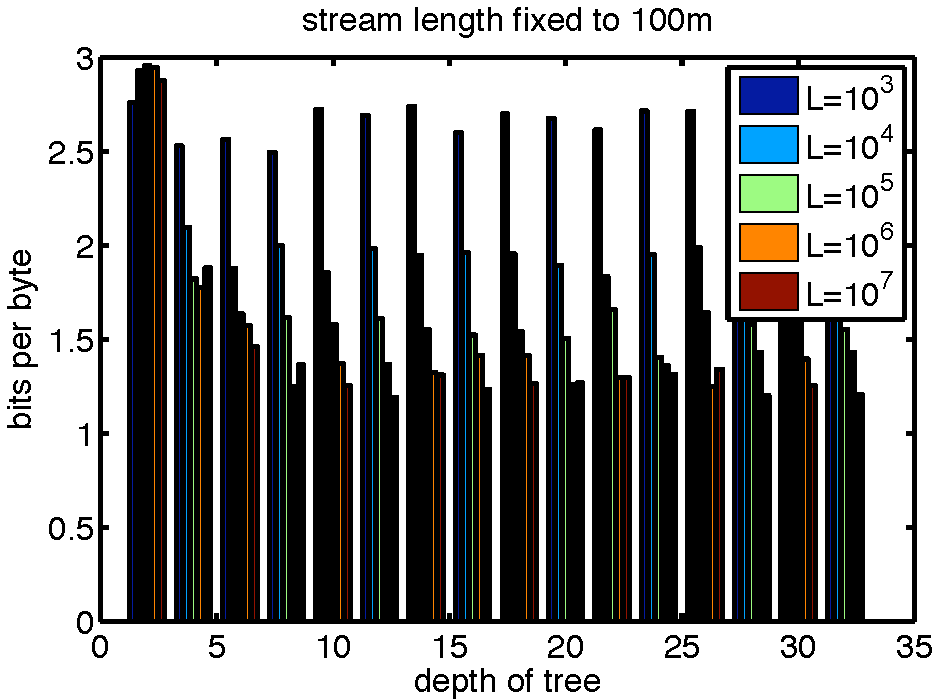
\includegraphics{figs/varying_depths.pdf}} % [clip=true, viewport= 1in 1in 9in 9in]
		\caption{Performance averaged over 10 random sections  100Mb sections of the corpus for varying fixed depths and number of allowable nodes ($L$) }
		\label{fig:varying_depths}
	\end{center} 
\end{figure*} 

%\begin{figure*}[t] 
%	\begin{center}
%		\scalebox{.6}{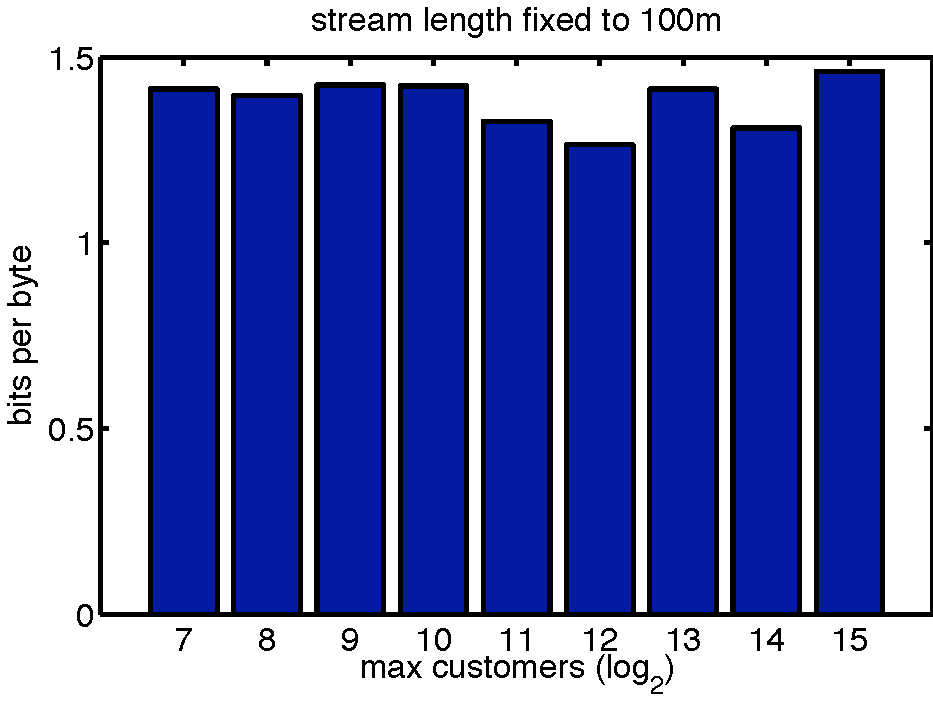
\includegraphics{figs/varying_max_customers.pdf}} % [clip=true, viewport= 1in 1in 9in 9in]
%		\caption{Performance for varying max allowable customers $k$.}
%		\label{fig: varying_max_customers}
%	\end{center} 
%\end{figure*} 

\begin{figure*}[t] 
	\begin{center}
		\scalebox{.6}{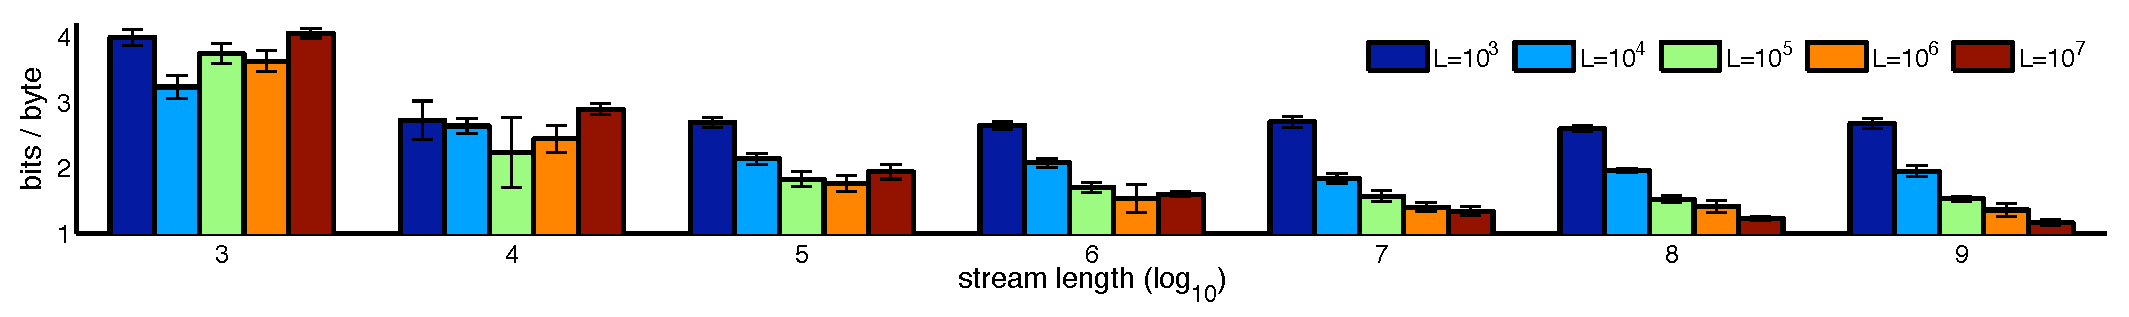
\includegraphics{figs/varying_stream_length.pdf}} % [clip=true, viewport= 1in 1in 9in 9in]
		\caption{Performance for varying stream lengths and number of allowable nodes ($L$).}
		\label{fig:varying_stream_length}
	\end{center} 
\end{figure*} 


%\begin{figure*}[t] 
%	\begin{center}
%		\scalebox{1}{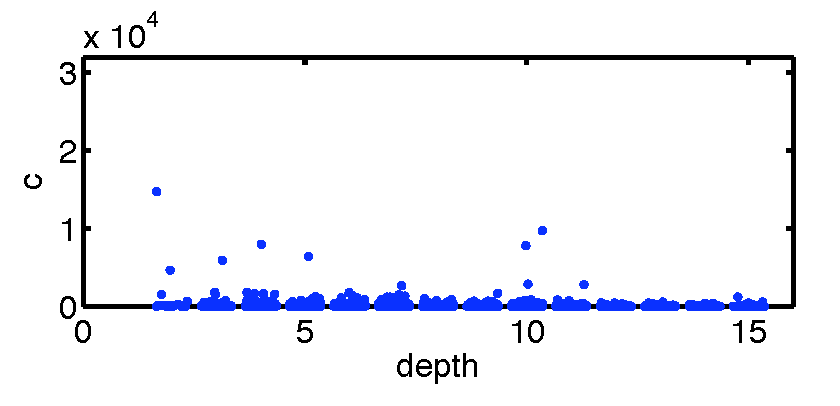
\includegraphics{figs/scatter_16.pdf}} % [clip=true, viewport= 1in 1in 9in 9in]
%		\caption{Scatter plots to explore the relationship between the depth of a node and the total count}
%		\label{fig:restaurant_plots}
%	\end{center} 
%\end{figure*} 

%\begin{figure*}[t] 
%	\begin{center}
%		\scalebox{1}{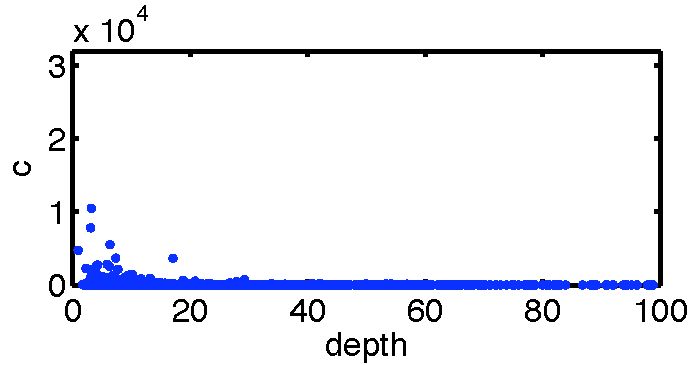
\includegraphics{figs/scatter_1024.pdf}} % [clip=true, viewport= 1in 1in 9in 9in]
%		\caption{Scatter plots to explore the relationship between the depth of a node and the total count}
%		\label{fig:restaurant_plots}
%	\end{center} 
%\end{figure*} 

\section{Discussion}
\label{sec:discussion}
% !TEX root = main.tex
\section{Discussion}
\label{section_discussion}

Things to consider: 

1) Scaling to phrases.
2) Making the spelling correction parameterization context dependent.


 \bibliographystyle{plainnat} \bibliographystyle{plainnat}
\bibliographystyle{plainnat}
\bibliography{refs}

\end{document}  